%
% Diseño de operaciones en red
% Capítulo de análisis y diseño de api web.
% Proyecto Lovelace
%

\subsection{API web}

En la figura \ref{diagrama_api} se muestran las operaciones de la \gls{gl:api}.
Aunque más adelante se detallan algunas otras operaciones secundarias, la idea
general es solamente esta. El cliente de la \gls{gl:api} puede tokenizar un
número de tarjeta dado, mediante la \gls{gl:uri} de \texttt{/tokenizar}, o puede
hacer el proceso inverso, mediante la \gls{gl:uri} \texttt{/detokenizar}.

\begin{figure}
  \begin{center}
    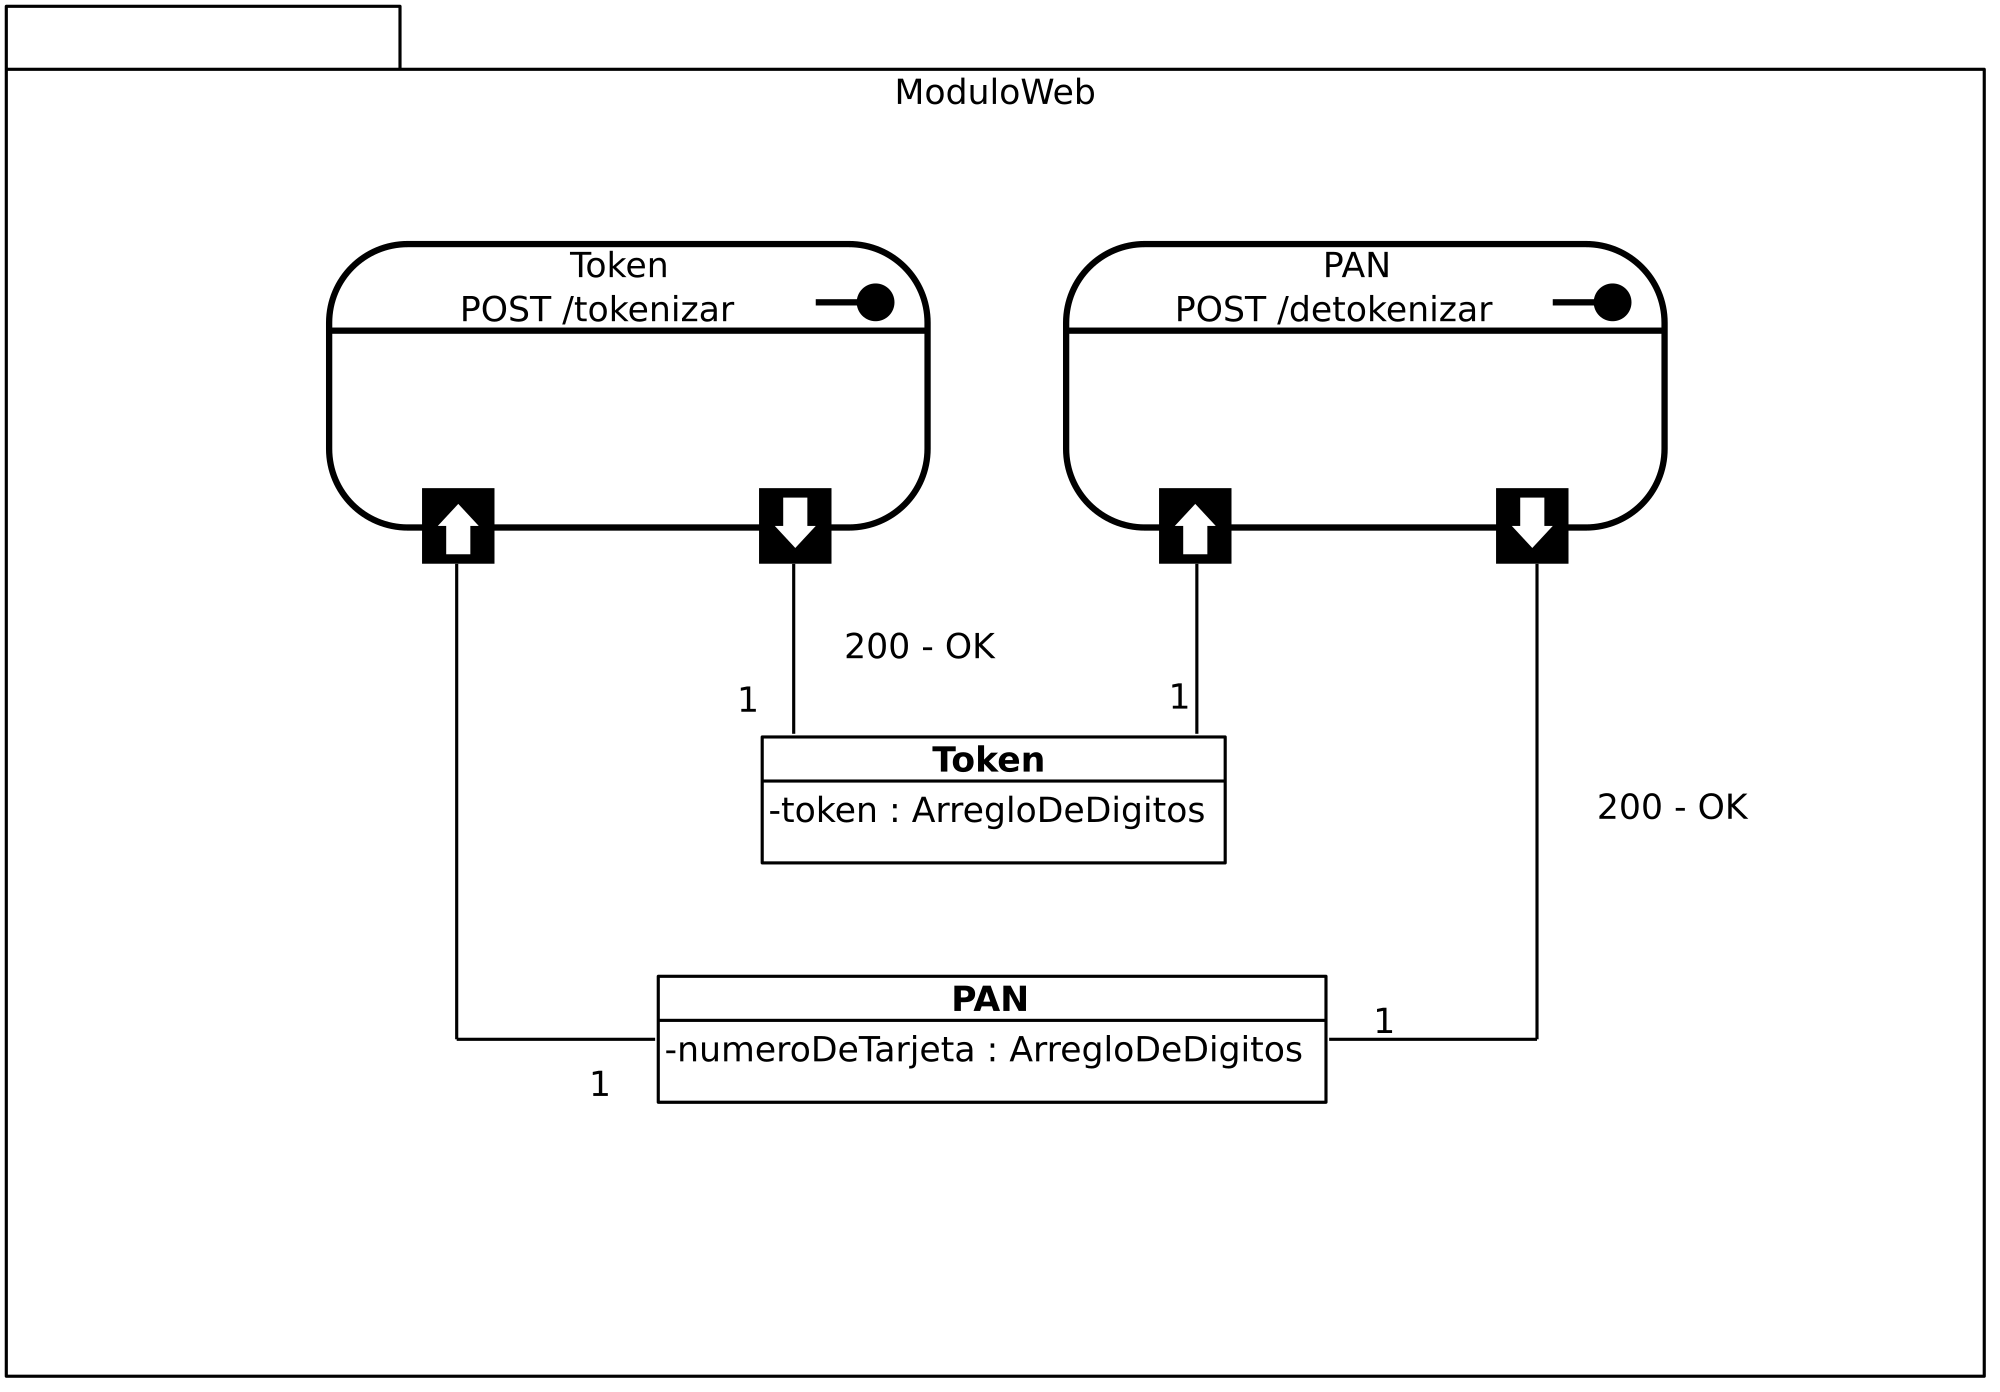
\includegraphics[width=0.8\linewidth]{diagramas/api_rest.png}
    \caption{Diagrama de recursos \gls{gl:rest}.}
    \label{diagrama_api}
  \end{center}
\end{figure}
